\documentclass[border=4pt]{standalone}
\usepackage{fontspec}
\usepackage{amsmath}
\usepackage{unicode-math}
\setmainfont{Latin Modern Roman}
\setmathfont{Latin Modern Math}
\usepackage{pgfplots}
\usepackage{pgfplotstable}
\pgfplotsset{compat=1.18}
\usepackage{tkz-euclide}
\usetikzlibrary{arrows.meta,calc,angles,quotes,patterns,3d,backgrounds}
\definecolor{ink}{HTML}{123428}
\definecolor{asy}{HTML}{475569}
\definecolor{mint}{HTML}{86e0bd}
\tikzset{asym/.style={asy, line width=0.9pt, dash pattern=on 5pt off 3.5pt},
         guide/.style={gray!70, line width=0.6pt, densely dotted},
         dot/.style={circle, inner sep=0pt, minimum size=5pt, draw=white, line width=0.5pt},
         odot/.style={circle, inner sep=0pt, minimum size=5.5pt, fill=white, line width=1pt},
         lab/.style={font=\footnotesize, inner sep=1.5pt, text=ink}}
\begin{document}
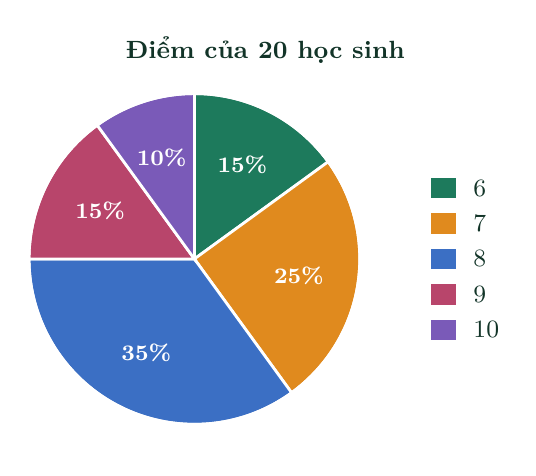
\begin{tikzpicture}[x=1cm, y=1cm]
\fill[fill={rgb,255:red,29;green,122;blue,92}, draw=white, line width=1pt] (0,0) -- (90.0000:2.1) arc[start angle=90.0000, end angle=36.0000, radius=2.1cm] -- cycle;
\node[font=\footnotesize\bfseries, text=white] at (63.0000:1.344) {15\%};
\fill[fill={rgb,255:red,224;green,138;blue,30}, draw=white, line width=1pt] (0,0) -- (36.0000:2.1) arc[start angle=36.0000, end angle=-54.0000, radius=2.1cm] -- cycle;
\node[font=\footnotesize\bfseries, text=white] at (-9.0000:1.344) {25\%};
\fill[fill={rgb,255:red,59;green,111;blue,196}, draw=white, line width=1pt] (0,0) -- (-54.0000:2.1) arc[start angle=-54.0000, end angle=-180.0000, radius=2.1cm] -- cycle;
\node[font=\footnotesize\bfseries, text=white] at (-117.0000:1.344) {35\%};
\fill[fill={rgb,255:red,184;green,69;blue,107}, draw=white, line width=1pt] (0,0) -- (-180.0000:2.1) arc[start angle=-180.0000, end angle=-234.0000, radius=2.1cm] -- cycle;
\node[font=\footnotesize\bfseries, text=white] at (-207.0000:1.344) {15\%};
\fill[fill={rgb,255:red,122;green,90;blue,184}, draw=white, line width=1pt] (0,0) -- (-234.0000:2.1) arc[start angle=-234.0000, end angle=-270.0000, radius=2.1cm] -- cycle;
\node[font=\footnotesize\bfseries, text=white] at (-252.0000:1.344) {10\%};
\draw[white, line width=1pt] (0,0) circle (2.1);
\fill[fill={rgb,255:red,29;green,122;blue,92}] (3.0,0.770) rectangle ++(0.32,0.26);
\node[anchor=west, font=\small, text=ink] at (3.42,0.900) {6};
\fill[fill={rgb,255:red,224;green,138;blue,30}] (3.0,0.320) rectangle ++(0.32,0.26);
\node[anchor=west, font=\small, text=ink] at (3.42,0.450) {7};
\fill[fill={rgb,255:red,59;green,111;blue,196}] (3.0,-0.130) rectangle ++(0.32,0.26);
\node[anchor=west, font=\small, text=ink] at (3.42,0.000) {8};
\fill[fill={rgb,255:red,184;green,69;blue,107}] (3.0,-0.580) rectangle ++(0.32,0.26);
\node[anchor=west, font=\small, text=ink] at (3.42,-0.450) {9};
\fill[fill={rgb,255:red,122;green,90;blue,184}] (3.0,-1.030) rectangle ++(0.32,0.26);
\node[anchor=west, font=\small, text=ink] at (3.42,-0.900) {10};
\node[font=\bfseries\small, text=ink] at (0.9,2.6500000000000004) {Điểm của 20 học sinh};
\end{tikzpicture}
\end{document}
